\chapter{Version Control}

\section{Software Versions}

No writer can finish a good book in one shot. A book needs to be
writen section by section and chapter by chapter. The writing is
likely reviewed and revised multiple times. If you watch a movie DVD,
you can find {\it Deleted Scenes}--- the sections that have been made
but never used in the actual movie.  Any non-trivial work needs to be
created gradually and improved over and over again before it is ready.
Developing software is no different: functionality is added
gradually. Sometimes, finished functions need to change because
customers' needs have changed, competitors have introduced new
features and modifications are needed, new regulations are announced,
or new standards are issued. All of these mean that software must be
developed in small pieces; these pieces are called {\it version}.

There is no widely accepted definition of a version, just like there
is no specific definition what should be considered as a chapter in a
book. One may consider each additional line as a new version while
another may consider a completely implemented and fully tested feature
as a version. Generally speaking, a version should be self-contained
and complete unit, like a section or a chapter in a book.  The tools
that manage versions are called {\it version control}.  When multiple
work together, version control becomes essential to ensure proper
coordination.

There are many version control systems, such {\tt CVS} (concurrent
version system) and {\tt SVN} (subversion).  This book uses {\tt git}
for version control. It is a {\it distributed} version control system,
meaning that there can be two types of {\it repositories}: One is on
each user's computer; the other is shared by all users. The advantage
of a distributed version control system will become clear after
explaining how people collaborate developing software.

The version control system {\tt git} is a set of programs managing
files.  You can run {\tt git} on your own computer. You can also set
up a {\tt git} server shared by multiple people. Alternatively, you
can use websites that offer version control functions; examples
include {\tt github.com} and {\tt bitbucket.org}.  This book uses {\tt
  github} as an example.  You can find entire books talking about {\tt
  git} as well as thousands of web postings about how to use {\tt
  github}. {\tt git} has many different functions and {\tt github}
offers many different ways to accomplish the same goals.  This book
does not intend to replace those materials.  Instead, this book
provides enough details for common needs.  Readers interested knowing
more can easily find additional documentations.
\marginnote{The authors are users of  {\tt github.com}
  and have no other connection with {\tt github.com}.}

\section{\tt github}

This book chooses {\tt github} for three reasons: (1) It is widely
used.  (2) It is free for education purposes. (3) It is supported by
many tools other than the {\tt github} website.
Figure~\ref{fig:github12} shows the website of {\tt github} and the
portal for an education account.

\begin{figure}[h] \centering
 \subfigure[]
{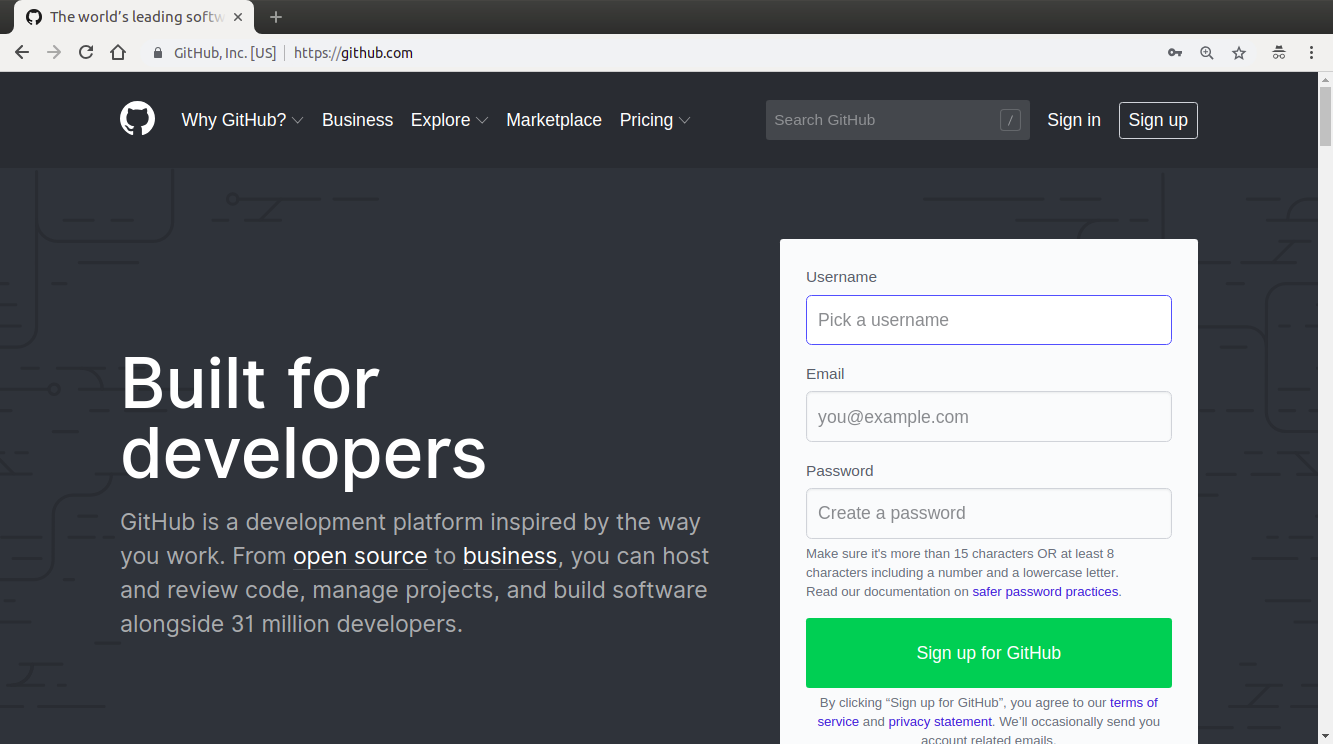
\includegraphics[width=4.5in]{\thischapterpath/figures/github1.png}}
  \subfigure[]
{
\includegraphics[width=4.5in]{\thischapterpath/figures/github2.png}}
\caption{(a) {\tt github} website. (b) Students and teachers can apply for free repositories.}
\label{fig:github12}
\end{figure}

Signing up in {\tt github} is easy, as shown in
Figure~\ref{fig:github34} (a).  After creating an account, a
repository can be created as shown in Figure~\ref{fig:github34} (b).
This website has many options: the name of the repository, whether it
is public or private, whether to initialize the repository with {\tt
  README}, etc.


\begin{figure}[h] \centering
 \subfigure[]
{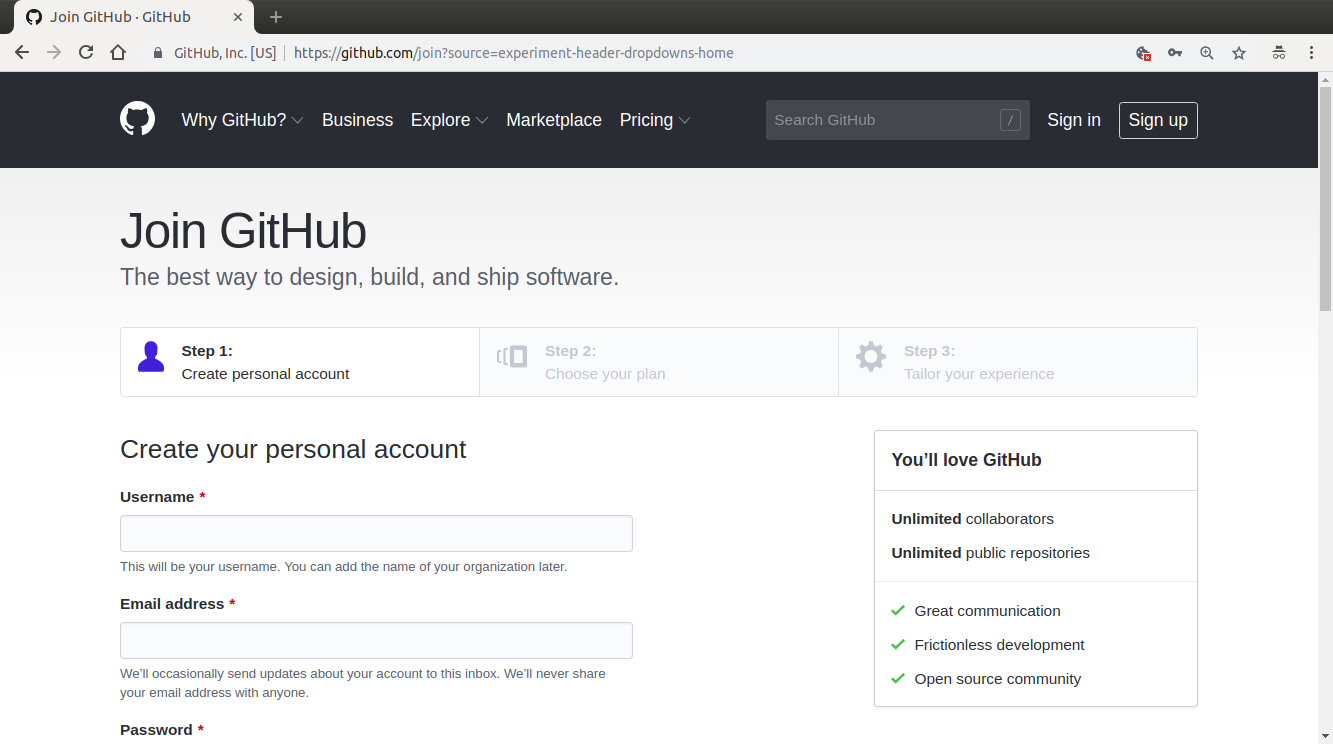
\includegraphics[width=4.5in]{\thischapterpath/figures/github3.png}}
  \subfigure[]
{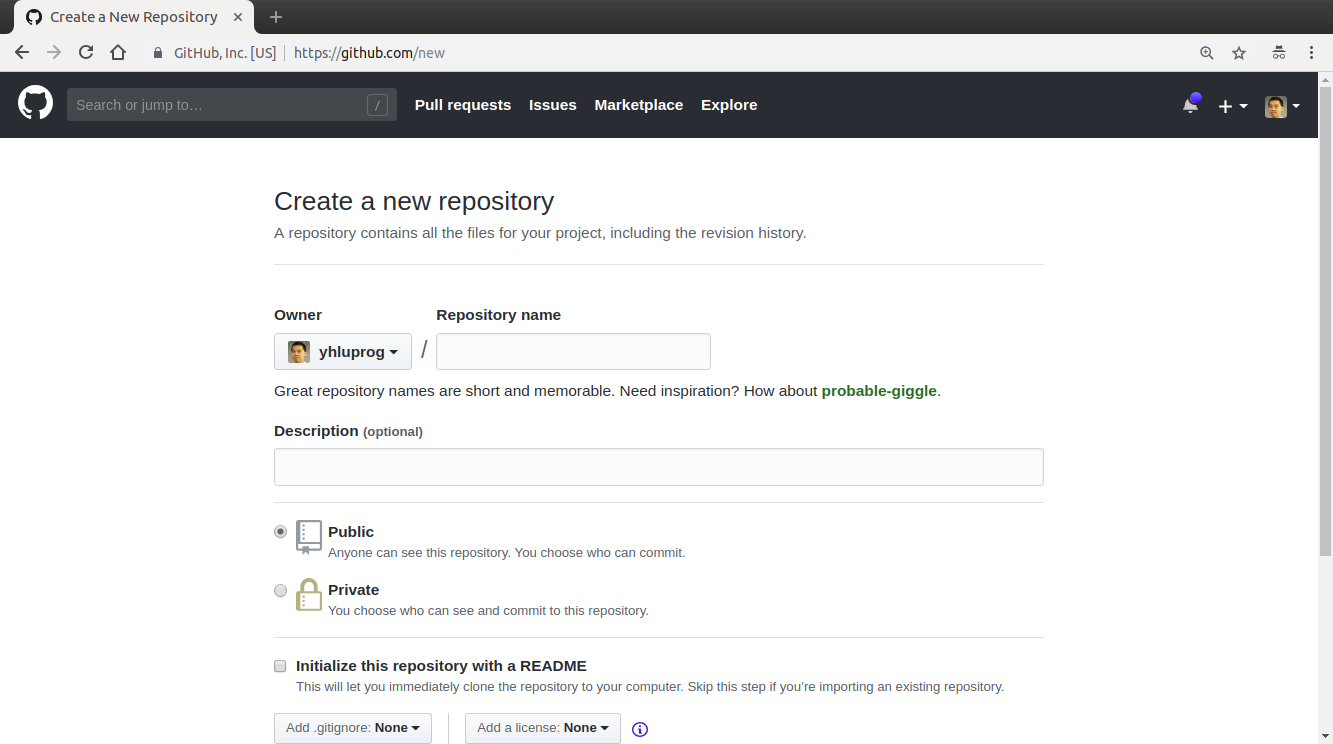
\includegraphics[width=4.5in]{\thischapterpath/figures/github4.png}}
\caption{(a) Create an account in {\tt github}. (b) Create a
  repository.}
\label{fig:github34}
\end{figure}

\begin{figure}[h] \centering
   \subfigure[]
{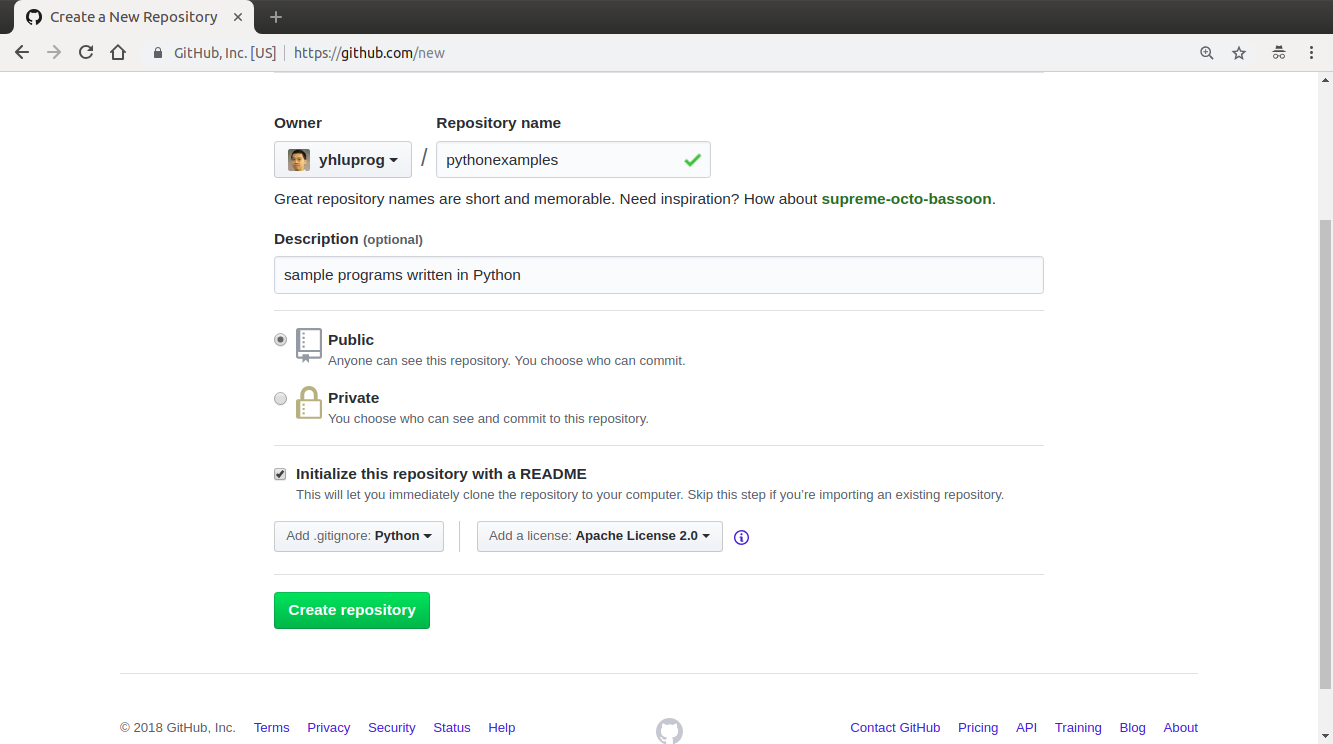
\includegraphics[width=4.5in]{\thischapterpath/figures/github5.png}}
   \subfigure[]
{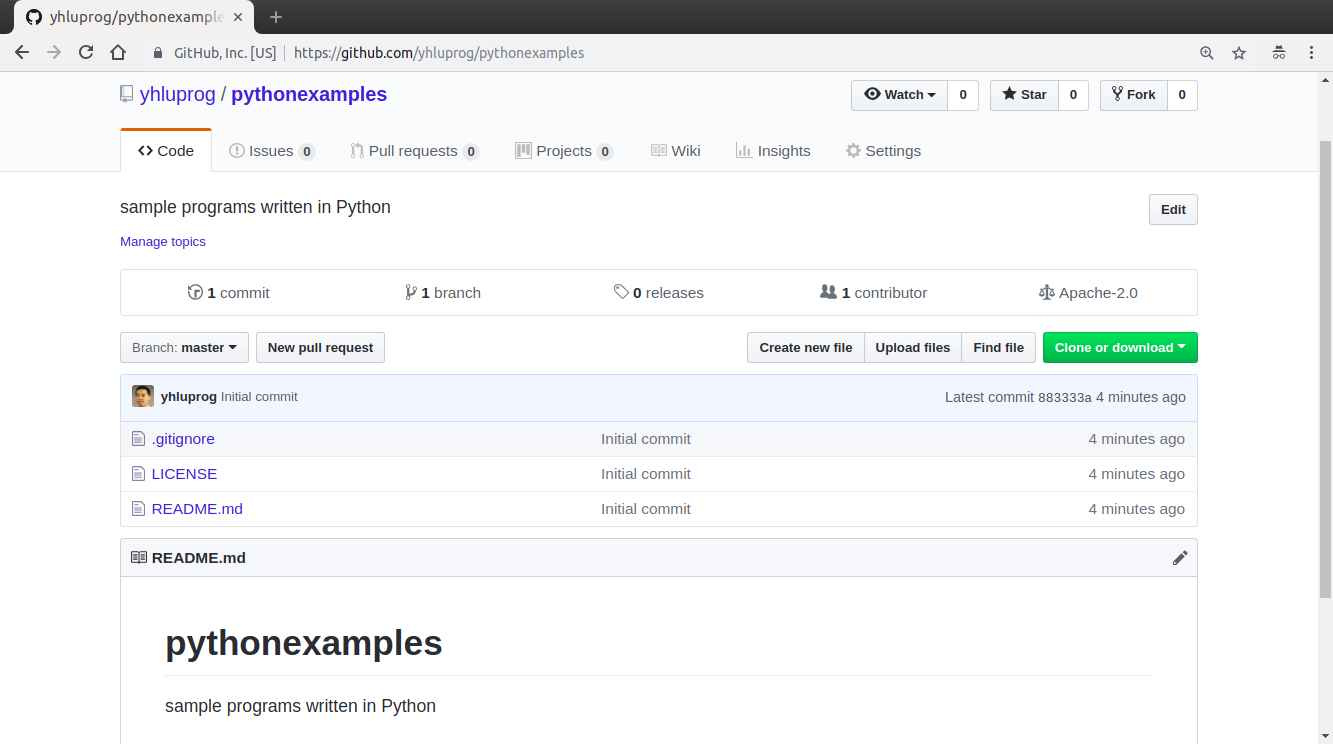
\includegraphics[width=4.5in]{\thischapterpath/figures/github6.png}}
\caption{(a) A new repository. (b) The repository has been created.}
\label{fig:github56}
\end{figure}

\marginnote{Is {\tt git} case sensitive? The correct answer
  is ``it is complicated''. A short answer is ``No'': you
  should treat {\tt git} as case insensitive. Do not have two
files whose names are different by cases only.}

Figure~\ref{fig:github56} (a) shows the options for creating a new repository:


\begin{itemize}
\item Repository name: pythonexamples
\item Description: sample programs written in Python
\item Public
\item Check ``Initialize this repository with a README''
\item Select ``Add .gitignore: Python''
\item Select ``Add a license: Apache License 2.0''
\end{itemize}


Figure~\ref{fig:github56} (b) shows the repository after it has been
created.  As can be seen on the website, there are many options
changing this repository.  For example, it is possible adding new
files or uploading files. It is also possible editing an file by
clicking the pen icon.

\section{Clone a Repository}

A more common way of using a repository, however, is to {\it clone} the
repository on another computer, as illustrated in Figure~\ref{fig:gitclone}.

\index{git!clone}

\begin{figure}[h] \centering
{
\includegraphics[width=3in]{\thischapterpath/figures/gitclone.png}}
\caption{Using {\tt git clone} command creates a repository on another computer.}
\label{fig:gitclone}
\end{figure}

To clone a repository, it is necessary knowing the {\it path} in {\tt
  github}.  Figure~\ref{fig:github7} shows the path of the repository.

\begin{figure}[h] \centering
{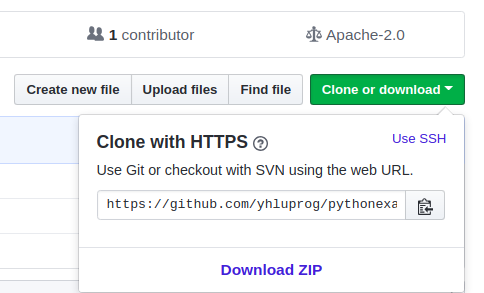
\includegraphics[width=3in]{\thischapterpath/figures/github7.png}}
\caption{Cloning a repository may use HTTPS or SSH.}
\label{fig:github7}
\end{figure}


\clearpage

\index{git!clone}
To clone the repository, starts a {\it Terminal} in Linux
and type the {\tt git clone} command. In the following
example, {\tt \$} is the {\it command prompt} for the Terminal.

\vspace{0.2in}

\noindent
\begin{tabular}{|p{5in}|}\hline
\begin{verbatim}
$ git clone https://github.com/yhluprog/pythonexamples.git
\end{verbatim}
\\ \hline
\end{tabular}
\vspace{0.2in}

The command clones the repository and the following message is shown:

\vspace{0.2in}

\noindent
\begin{tabular}{|p{5in}|}\hline
\begin{verbatim}
Cloning into 'pythonexamples'...
remote: Enumerating objects: 5, done.
remote: Counting objects: 100% (5/5), done.
remote: Compressing objects: 100% (5/5), done.
remote: Total 5 (delta 0), reused 0 (delta 0), pack-reused 0
Unpacking objects: 100% (5/5), done.
Checking connectivity... done.
\end{verbatim}
\\ \hline
\end{tabular}
\vspace{0.2in}

After cloning the repository, a directory (also called folder) with
the name {\tt pythonexamples} is created.  This can be shown
using the {\tt ls} command:

\vspace{0.2in}

\noindent
\begin{tabular}{|p{5in}|}\hline
\begin{verbatim}
$ ls
pythonexamples/
\end{verbatim}
\\ \hline
\end{tabular}
\vspace{0.2in}

Inside this directory, there are already two files: {\tt
  LICENSE} and {\tt README.md}. The is a hidden file {\tt .gitignore}.
It is hidden because it starts with {\tt .} and is not shown by the
{\tt ls} command. To show a hidden file, it is necessary using the
{\tt ls -a} command. Additionally, a hidden directory (ending with
{\tt /}) called {\tt .git} is also shown.

\vspace{0.2in}

\noindent
\begin{tabular}{|p{5in}|}\hline
\begin{verbatim}
$ cd pythonexamples/
$ ls -a
./  ../  .git/	.gitignore  LICENSE  README.md
\end{verbatim}
\\ \hline
\end{tabular}
\vspace{0.2in}

Enter the directory using the {\tt cd} command
and use the {\tt ls} command to see the files and directories.

\vspace{0.2in}

\noindent
\begin{tabular}{|p{5in}|}\hline
\begin{verbatim}
$ cd .git
$ ls
branches/  config  description	HEAD  hooks/  index  
info/  logs/  objects/  packed-refs  refs/
\end{verbatim}
\\ \hline
\end{tabular}
\vspace{0.2in}


Among them, {\tt config} stores the information about
the remote repository.  The {\tt more} command can show
the content of the file:

\vspace{0.2in}

\noindent
\begin{tabular}{|p{5in}|}\hline
\begin{verbatim}
$ more config
[core]
	repositoryformatversion = 0
	filemode = true
	bare = false
	logallrefupdates = true
[remote "origin"]
	url = https://github.com/yhluprog/pythonexamples.git
	fetch = +refs/heads/*:refs/remotes/origin/*
[branch "master"]
	remote = origin
	merge = refs/heads/master
\end{verbatim}
\\ \hline
\end{tabular}
\vspace{0.2in}

\index{git!clone}
The line starting with {\tt url} is the path used in {\tt git clone}.
The concept of {\it branch} will be explained later in this chapter.

\section{Commit and Push}

\marginnote{Modifying {\tt LICENSE} is not recommended.}

There are many different methods modifying a repository.  The first
method modifies an existing file.  Use a text editor and add the
following line to {\tt README.md}:

\begin{verbatim}
This repository demonstrates how to use commit, push, and branch.
\end{verbatim}

\index{git!commit}
After adding this line, use the {\tt git commit} command to show which file
has been changed:

\vspace{0.2in}

\noindent
\begin{tabular}{|p{5in}|}\hline
\begin{verbatim}
$ git commit
On branch master
Your branch is up-to-date with 'origin/master'.
Changes not staged for commit:
	modified:   README.md
\end{verbatim}
\\ \hline
\end{tabular}
\vspace{0.2in}

What does this mean? It says a file {\tt README.md} has been changed
but it has not been committed. The next question is the difference
between changes and commit.  Modifications are often reviewed and
revised multiple times; these changes are transient and do not need to
be recorded in the repository.  When the modifications are
satisfactory, the file is ready to ``take a snapshot'' by creating a
new version.  The command to take a snapshot is {\tt git commit}.
\index{git!commit}

The earlier {\tt git commit} shows the candidate(s) for commit.  A
candidate can be a files that has been modified ({\tt README.md} in
this example).  This command has not committed any changes yet and has
not created a new version. To commit the change of a specific file, it
is necessary adding the file's name as shown in the following example

\vspace{0.2in}

\noindent
\begin{tabular}{|p{5in}|}\hline
\begin{verbatim}
$ git commit -m "add a line" README.md 
[master 26317f0] add a line
 1 file changed, 2 insertions(+)
\end{verbatim}
\\ \hline
\end{tabular}
\vspace{0.2in}

\marginnote{It is a good habit of using meaningful commit
  messages because these messages can be searched to
  find the right version.}

In this command, {\tt -m} means the commit message and this commit
message is ``add a line''.  The name of the file, {\tt README.md}, is
included to indicate which file to take a snapshot and a new version
is created.

\index{git!commit}
\begin{figure}[h] \centering
{
\includegraphics[width=2.5in]{\thischapterpath/figures/gitcommit.png}}
\caption{After several changes, {\tt git commit} creates a new version
  and store it in the local repository.}
\label{fig:gitcommit}
\end{figure}

This new version is visible at only the local repository, not the remote
repository (in {\tt github}).  To make the changes visible in {\tt github},
another command {\tt git push} is needed.
\index{git!push}

\vspace{0.2in}

\noindent
\begin{tabular}{|p{5in}|}\hline
\begin{verbatim}
$ git push
Username for 'https://github.com': yhluprog
Password for 'https://yhluprog@github.com': 
Counting objects: 3, done.
Delta compression using up to 4 threads.
Compressing objects: 100% (3/3), done.
Writing objects: 100% (3/3), 343 bytes | 0 bytes/s, done.
Total 3 (delta 1), reused 0 (delta 0)
remote: Resolving deltas: 100% (1/1), completed with 1 local object.
To https://github.com/yhluprog/pythonexamples.git
   883333a..26317f0  master -> master
\end{verbatim}
\\ \hline
\end{tabular}
\vspace{0.2in}

\marginnote{A public repository (or open-source) repository allows
  everyone to read but only permitted people (determined by the owner
  of the repository) can write.}

\index{git!push}
\index{git!commit}
The {\tt git push} command needs an user name and the password because
it does not allow everyone to push and modify the repository.  The
rest of the message can be ignored for now.  Figure~\ref{fig:gitpush}
shows the typical workflow of using {\tt github}: Use {\tt git push}
to modify the remote repository after several {\tt git commit}
commands creating new versions on the local repository.

\begin{figure}[h] \centering
{
\includegraphics[width=2.5in]{\thischapterpath/figures/gitpush.png}}
\caption{Typical workflow of using {\tt github}}
\label{fig:gitpush}
\end{figure}

\clearpage

Figure~\ref{fig:github8} shows the {\tt github} website after {\tt git
  push}.  The changes are clearly marked: if a new line is added, a
``+'' sign is added in front.  Similarly, if a line is deleted, a
``-'' sign is added in front (not shown in this example).

\begin{figure}[h] \centering
{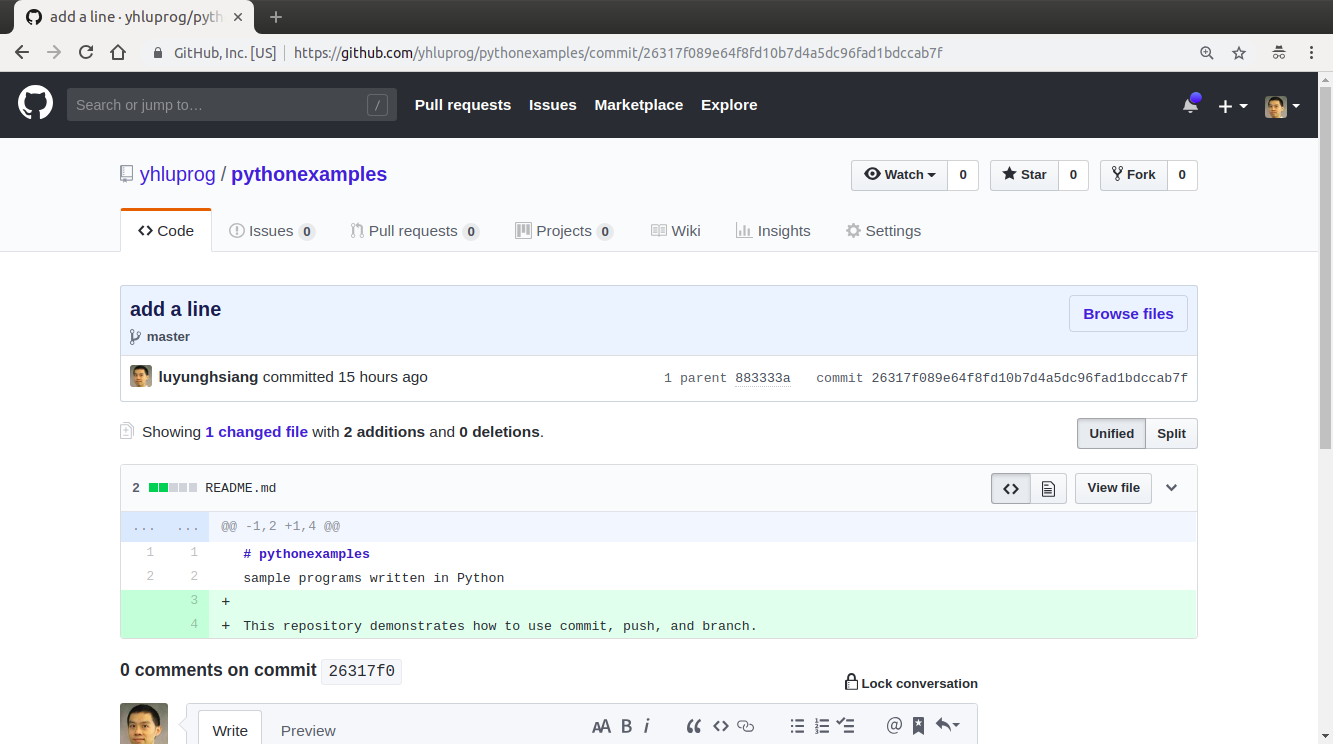
\includegraphics[width=4.5in]{\thischapterpath/figures/github8.png}}
\caption{The website of {\tt github} shows the change.}
\label{fig:github8}
\end{figure}


\section{Add and Remove Files}

The examples so far only modify an existing file: {\tt README.md}
added by {\tt github} when the repository is created.  This section
explains how to add and remove files or directories.  Use a text
editor to create the following simple Python program (without the line
numbers).

\resetlinenumber[1]
\linenumbers
\begin{tt}
  \lstinputlisting{\thischapterpath/code/hello.py}
\end{tt}
\nolinenumbers

\index{git!add}
\index{git!commit}

The {\tt git add} command informs the intention of adding this file to
the repository.  It is important to know that this file has not been
added yet.  To actually add this file, it is necessary using
the {\tt git commit} command followed by a message and the name of
the file to be added, as shown below.

\vspace{0.2in}

\noindent
\begin{tabular}{|p{5in}|}\hline
\begin{verbatim}
$ git add hello.py
$ git commit -m "add a new file to print hello" hello.py
[master 1ed761d] add a new file to print hello
 1 file changed, 7 insertions(+)
 create mode 100755 hello.py
\end{verbatim}
\\ \hline
\end{tabular}
\vspace{0.2in}

The {\tt git push} command modifies the repository in {\tt github}

\vspace{0.2in}
\noindent
\begin{tabular}{|p{5in}|}\hline
\begin{verbatim}
$ git push
Username for 'https://github.com': yhluprog
Password for 'https://yhluprog@github.com': 
Counting objects: 3, done.
Delta compression using up to 4 threads.
Compressing objects: 100% (3/3), done.
Writing objects: 100% (3/3), 365 bytes | 0 bytes/s, done.
Total 3 (delta 1), reused 0 (delta 0)
remote: Resolving deltas: 100% (1/1), completed with 1 local object.
To https://github.com/yhluprog/pythonexamples.git
   26317f0..1ed761d  master -> master
\end{verbatim}
\\ \hline
\end{tabular}
\vspace{0.2in}

\begin{figure}[h] \centering
{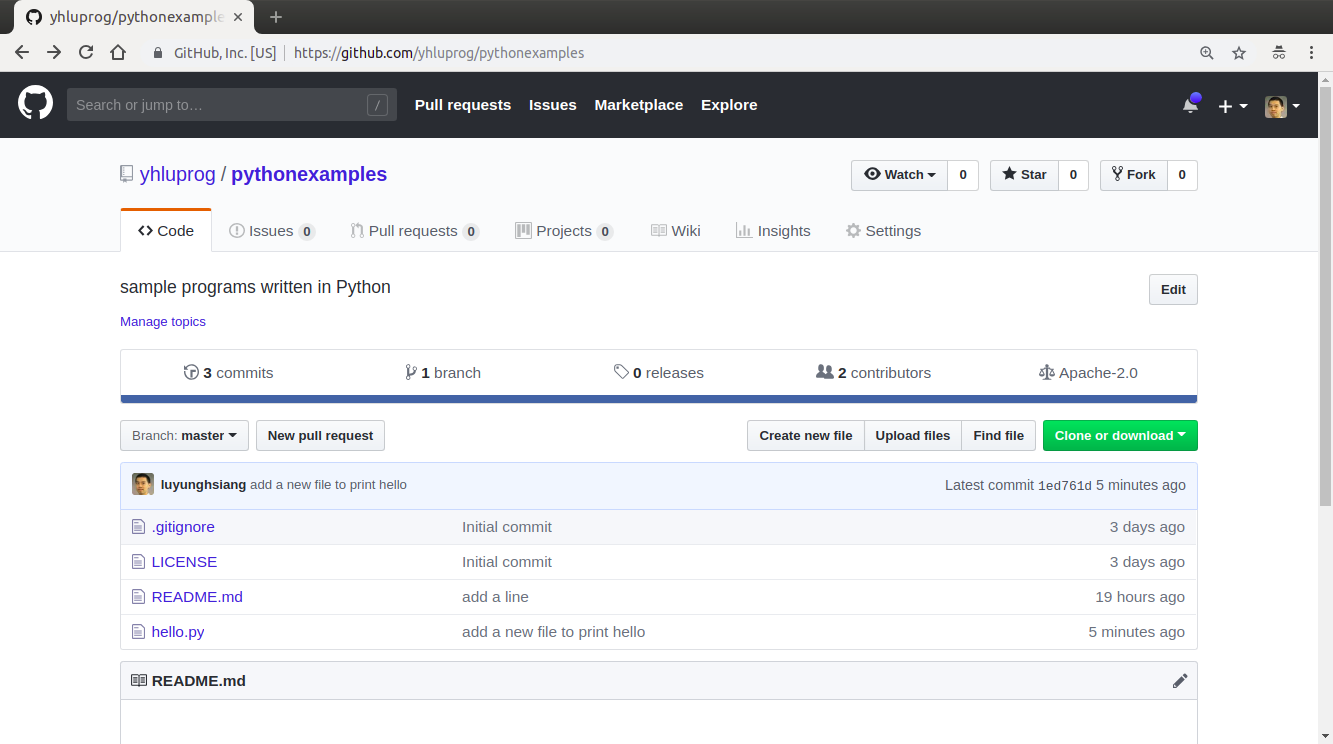
\includegraphics[width=4.5in]{\thischapterpath/figures/github10.png}}
\caption{The added file {\tt hello.py} is listed in {\tt github}.}
\label{fig:github10}
\end{figure}

A directory can be created using the {\tt mkdir} command in
Linux. Adding a file in a directory automatically to the repository
adds the directory.

To remove a file, use the {\tt git rm} command, followed by {\tt git commit}.
If {\tt git push} is used, the file is also removed from {\tt github}.

\vspace{0.2in}
\noindent
\begin{tabular}{|p{5in}|}\hline
\begin{verbatim}
$ git rm hello.py
rm 'hello.py'
$ git commit -m "remove the file" hello.py
[master 3357bae] remove the file
 1 file changed, 7 deletions(-)
 delete mode 100755 hello.py
$ git push
Username for 'https://github.com': yhluprog
Password for 'https://yhluprog@github.com': 
Counting objects: 2, done.
Delta compression using up to 4 threads.
Compressing objects: 100% (2/2), done.
Writing objects: 100% (2/2), 221 bytes | 0 bytes/s, done.
Total 2 (delta 1), reused 0 (delta 0)
remote: Resolving deltas: 100% (1/1), completed with 1 local object.
To https://github.com/yhluprog/pythonexamples.git
   1ed761d..3357bae  master -> master
\end{verbatim}
\\ \hline
\end{tabular}
\vspace{0.2in}

It is important to know that the deleted file does not disappear. It is still
stored in the history of the repository. In {\tt github}, clicking the commit
history shows all the changes over time, as shown in Figure~\ref{fig:github11}.

\begin{figure}[h] \centering
{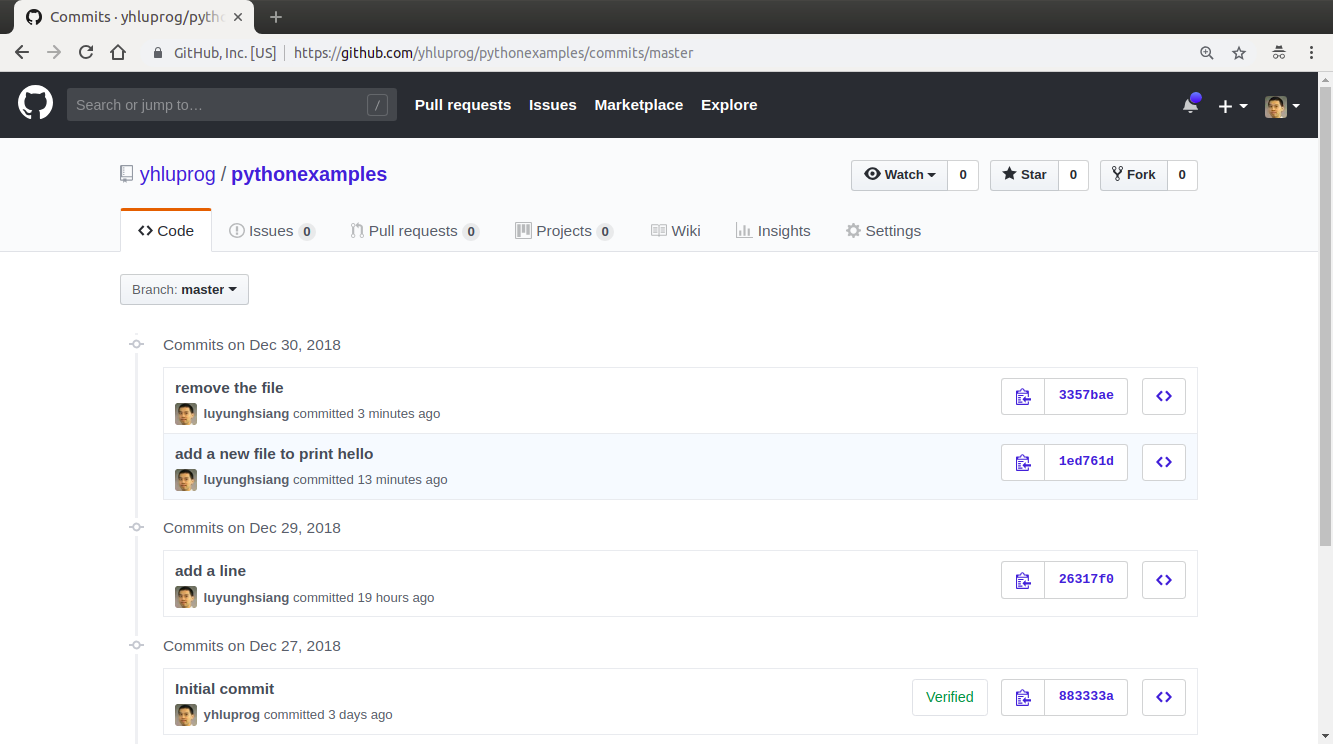
\includegraphics[width=4.5in]{\thischapterpath/figures/github11.png}}
\caption{The commit history.}
\label{fig:github11}
\end{figure}

\index{git!log}
It is also possible using the {\tt git log} command to see the history in
the reverse chronological order (the most recent first):

\vspace{0.2in}
\noindent
\begin{tabular}{|p{5in}|}\hline
\begin{verbatim}
$  git log
commit 3357baed98088aacc452a1135ff16739fe64cab6
Author: XXXX
Date:   YYYY

    remove the file

commit 1ed761dbd9a70c6b38a7d788dd3afc19d33f3b9a
Author: XXXX
Date:   YYYY

    add a new file to print hello

commit 26317f089e64f8fd10b7d4a5dc96fad1bdccab7f
Author: XXXX
Date:   YYYY

    add a line

commit 883333a9c3177b5e3d826addb15b8ebf4caf7b8c
Author: XXXX
Date:   YYYY

    Initial commit
\end{verbatim}
\\ \hline
\end{tabular}
\vspace{0.2in}


\section{Collaboration using {\tt github}}

Does does ``hub'' in {\tt github} mean? Think of it as an airline hub
or a bus hub, where travellers come from many different places in
order to change flights or bus lines.  Similarly, {\tt github} allows
collaborate to share and exchange.  Adding collaborators would be
easy, by clicking {\tt Settings} and {\tt Collaborators}, as shown
in Figure~\ref{fig:github9}.


\begin{figure}[h] \centering
{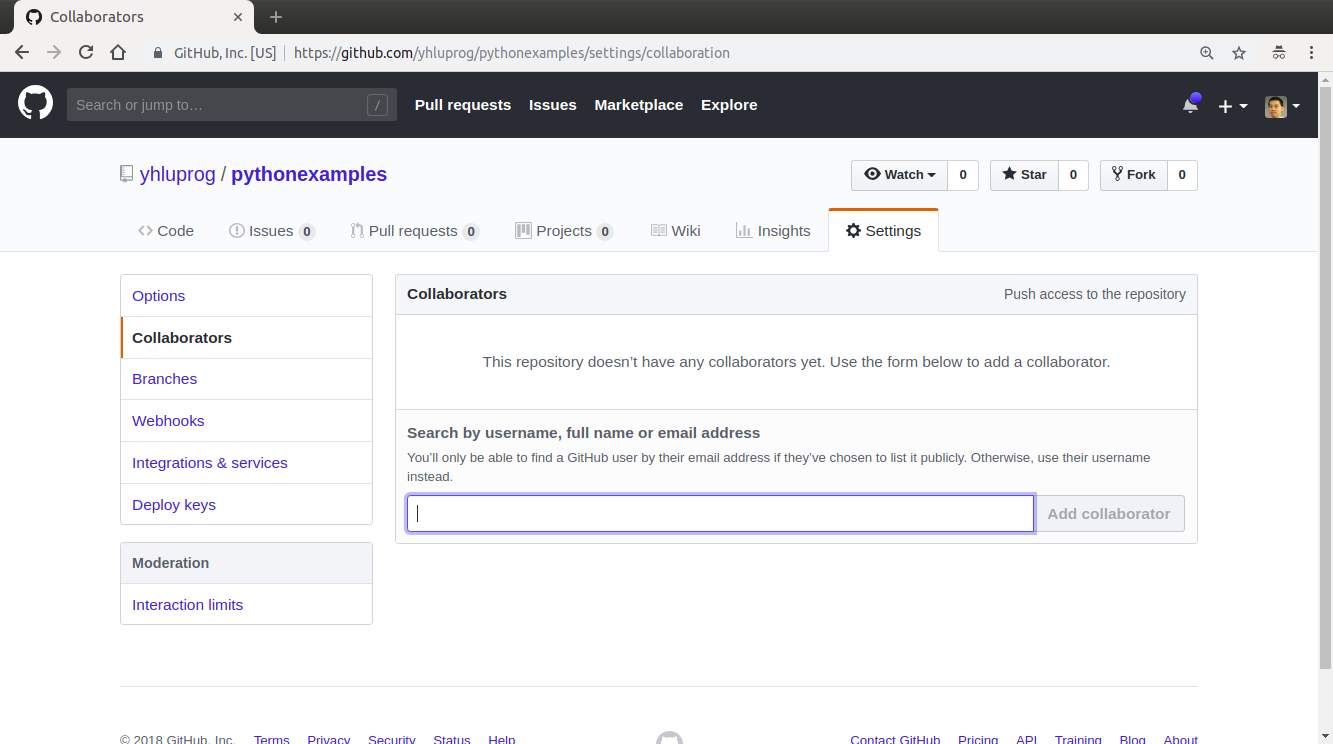
\includegraphics[width=4.5in]{\thischapterpath/figures/github9.png}}
\caption{Add collaborators to a repository.}
\label{fig:github9}
\end{figure}

Two people may share and modify the same repository in {\tt github} in
the way depicted in Figure~\ref{fig:githubcollaborate}.  In this
figure, the numbers in black ovals indicate steps within individual's
local repository.  The numbers in white ovals indicate steps involving
the remote repository.

\marginnote{Always do {\tt git pull} before {\tt git push}, unless it is already
  known that nobody has pushed since a repository is cloned.}

Each person starts by cloning the same repository in {\tt
  github}. After cloning, each person can work independently without
interfering with each other. Each person can also commit multiple
times creating multiple versions on their local repositories.  When
one decides it is time to share a version with the other person, this
version is pushed to the shared repository in {\tt github}.  Before
anything is pushed, the local repository should be updated by using
the {\tt git pull} command to ensure any changes by the other person
is reflected. Otherwise, the changes by the other person may be erased
by the new push.  Even though the erased changes can be recovered,
pushing without pulling first creates unnecessary trouble and is
impolite.

\index{git!pull}

Now is a good time explaining the advantage of distributed version
control systems like {\tt git}.  Figure~\ref{fig:githubcollaborate}
shows three repositories: one remote and shared in {\tt github} and
two local repositories by two different people. These two people can
change the files on their local repositories without affecting the
other person.  In fact, they can commit many times creating multiple
versions before pushing any changes and make the changes visible to
the other person.  An obvious question is when one should commit
and when one should push.

The answer to the first question is simple: commit anytime as one
wishes.  Since commit does not affect the shared repository, it is
acceptable committing changes that are incomplete or even contain
errors (i.e., ``bugs''). Committing creates a new version with a
message; this new version is searchable by the message.  When one
decides the changes are ``good enough'' to stay for now, it is time to
commit and create a new version.  

\begin{figure}[h] \centering
{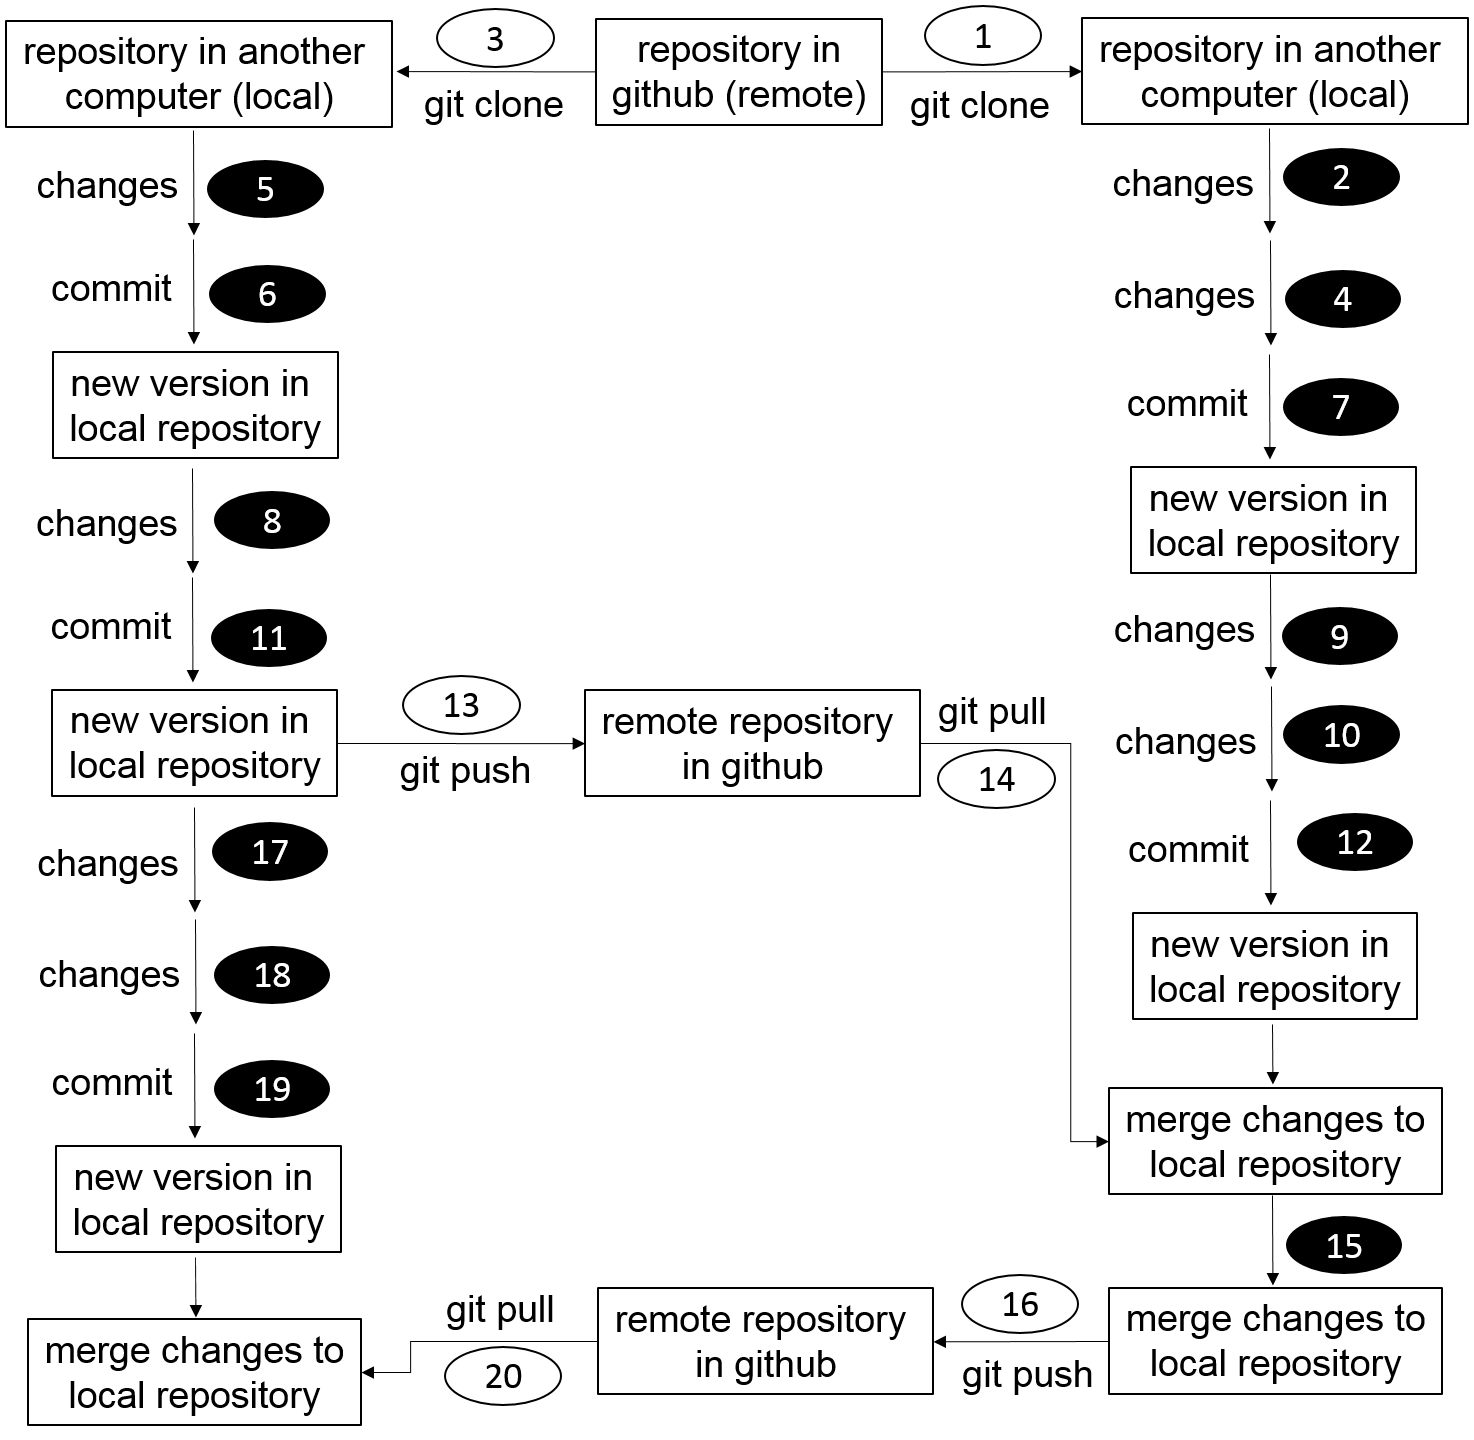
\includegraphics[width=4.5in]{\thischapterpath/figures/githubcollaborate.png}}
\caption{Workflow of two people upading the same repository in {\tt github}.}
\label{fig:githubcollaborate}
\end{figure}

In most cases, no problem occurs when two or more people modify the
same remote repository. If one person modifies a file another person
modifies a different file, {\tt git} simply takes the changes by both
people in the latest version.  Even if two people modify the same
file, {\tt git} may still be able to add the changes from both people.
In rare cases, however, {\it conflicts} may occur when two people
modify the same file and the changes are too similar for {\tt git} to
determine what to do.  Conflicts appear in th the following markers.

\begin{verbatim}
<<<<<<< 
content from one version
=======
content from the other version
>>>>>>> 
\end{verbatim}

\marginnote{The primary reason of conflicts is the lack of
  communication and coordination. Thus, the best way to avoid
  conflicts is to improve communication among the people modifying the
  same {\tt github} repository.}

Conventionally, the person that wants to push later is responsible
discovering and resolving conflicts.
